\subsubsection{Introduction}
%LET'S GO TEAM!!! ONE LESS SECTION
%We are unstoppppable --> DAB DAB DAB

In this section a first aproach of the drag computation have been done in order to determine the orbit decay and consequently compute how much time a satellite last untill it reenters the Earth atmosphere.

\subsubsection{Drag Computation Algorithm}

Given the definitions to calculate orbital perturbations described in \ref{TypesPerturb} a computation of the atmosphere drag has been done together with the computation of the other main perturbations that have been discussed in previous sections.

As explained in the last section the atmospheric drag depens on the drag's coefficient and it surface, that are constant values, on the velocity at which the satellite operates and on the air density.

So in order to see the effects of variations in air density the orbit decay has been estimated and plotted for several F10 Radio Flux values corresponding to different moments of a solar cycle. (This data has been extracted from the figure~\ref{solar}).

The data selected and the results obtained are shown in \ref{OrbDecCompT} and \ref{fig:OrbitDecayComp} respectively.


\begin{table}[]
\centering

\begin{tabular}{|l|c|}
\hline
\multicolumn{2}{|l|}{Selected Values}      \\ \hline
Year & \multicolumn{1}{l|}{F10 Radio Flux} \\ \hline
2002 & 195                                 \\ \hline
2004 & 115                                 \\ \hline
2009 & 70                                  \\ \hline
2013 & 120                                 \\ \hline
2016 & 100                                 \\ \hline
\end{tabular}
\caption{Selected data to compute orbit decay extracted from figure \ref{solar}}
\label{OrbDecCompT}
\end{table}  
\begin{figure}[H] %[b] % h / H / b / t
\centering
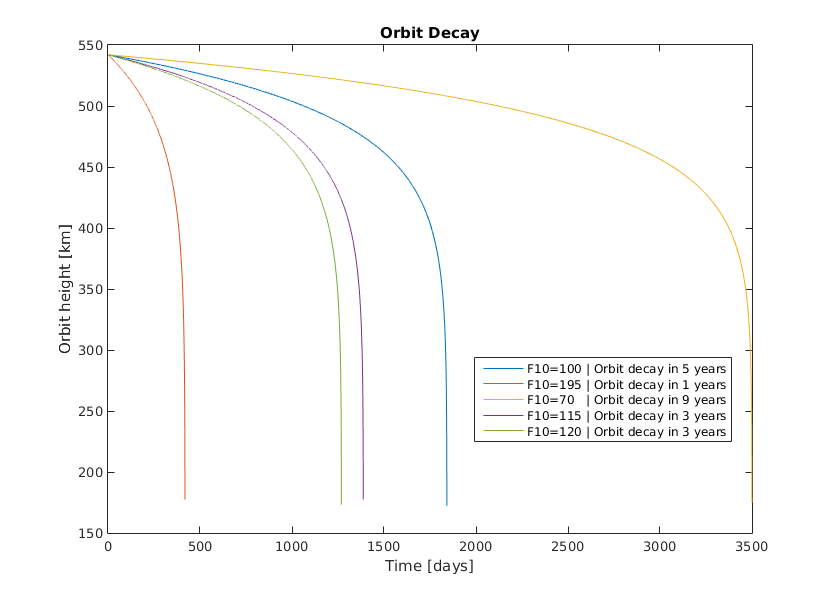
\includegraphics[width=.8\textwidth]{OrbitDecayComp.png}
\caption{Orbit Decay computed for several values of F10 Radio Flux}
\label{fig:OrbitDecayComp}
\end{figure}

As it can be seen, the orbit decay strongly depends on the positioning in time of a solar cycle. (In 7 years the difference in lasting time of the satellite is reduced in 4 years).

\paragraph{In conclusion}
The lasting time in orbit of satellites is affected by period of the solar cycle. According to the data then Astrea's satellites will have an approximated orbit decay of 5 years.


 